% !TEX root = keeping-up.tex


%%
\section{Figures}
\label{sec:figures}

Definitions of figures follows the environment definition like in \fref{fig:example}.
Figures should always use a meaningful description and be referenced in the text.

\begin{figure}
  \centering
  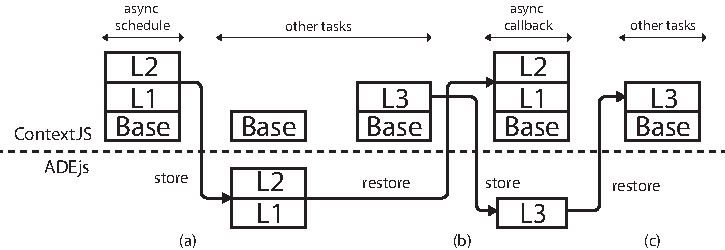
\includegraphics[width=0.75\columnwidth]{figures/approach}
  \caption{Figure description}
  \label{fig:example}
\end{figure}

Figures are floating elements, that means that latex will place them where they fit best. You can help the positioning by using the header placement options
\begin{description}[labelindent=1cm]
  \item[h] place the figure here
  \item[t] place the figure at the top of the page
  \item[b] place the figure at the bottom of the page
  \item[p] place the figure relative to this paragraph 
\end{description} 

There are multiple ways to place figures, inline, side-by-side, standalone, horizontally. The most common is to have them side-by-side and stand alone

\begin{figure}
\centering
\begin{subfigure}[b]{0.45\textwidth}
    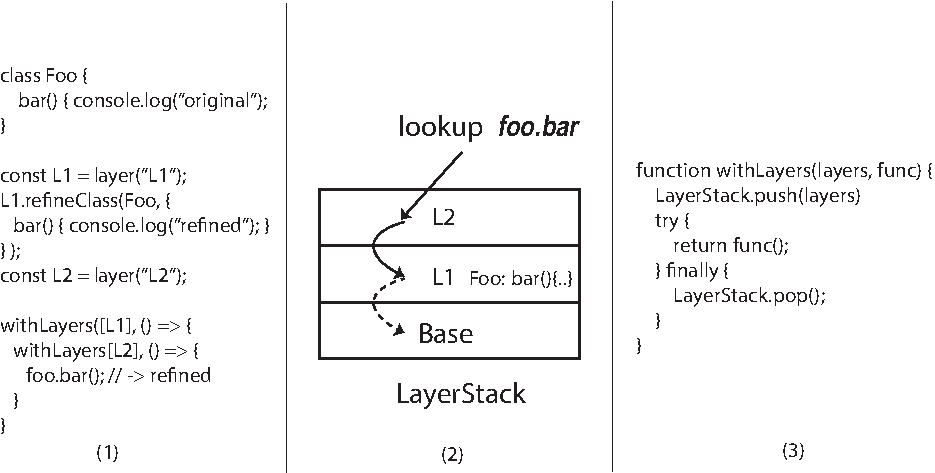
\includegraphics[width=\textwidth]{figures/contextjs}
    \caption{Firts subfigure.}
    \label{fig:first}
\end{subfigure}
\hfill
\begin{subfigure}[b]{0.45\textwidth}
    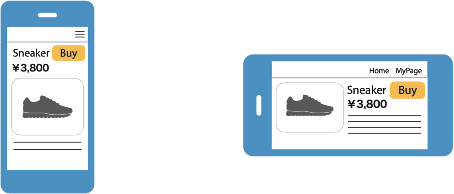
\includegraphics[width=\textwidth]{figures/copex2}
    \caption{Second subfigure.}
    \label{fig:second}
\end{subfigure}
\hfill
\begin{subfigure}{0.4\textwidth}
    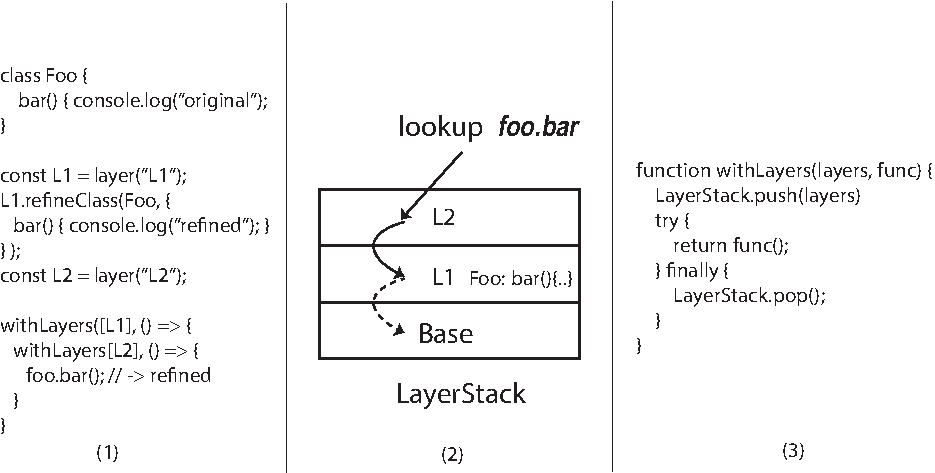
\includegraphics[width=\textwidth]{figures/contextjs}
    \caption{Third subfigure.}
    \label{fig:third}
\end{subfigure}
\caption{Subfigures side-by-side}
\label{fig:figures}
\end{figure}


Using this you can reference subfigures individually (\eg \fref{fig:first}, \fref{fig:second}, \fref{fig:third}) or altogether using the general label \fref{fig:figures}

\endinput